%Florian Bogner & Alexander Palmrich

\documentclass[a4paper,10pt,notitlepage,fullpage]{paper}
\usepackage{fullpage}
\usepackage[utf8]{inputenc}
%\usepackage[ngerman]{babel}
\usepackage[english]{babel}
\usepackage{amsmath}
\usepackage{amssymb}
\usepackage{latexsym}
\usepackage{mathtools}
\usepackage{listings}
\usepackage{algorithm}
\usepackage{algpseudocode}
\usepackage{graphicx}
\usepackage{booktabs}
\usepackage{hhline}
\usepackage{amsthm}
\usepackage{cite}
\usepackage{wrapfig}
\usepackage{hyperref}
\usepackage{titling}

\theoremstyle{plain}
\newtheorem{thm}{Theorem}[section] % reset theorem numbering for each chapter

\theoremstyle{definition}
\newtheorem{defn}[thm]{Definition} % definition numbers are dependent on theorem numbers
\newtheorem{exmp}[thm]{Example} % same for example numbers
\newtheorem{lem}[thm]{Lemma}
%https://tex.stackexchange.com/questions/45817/theorem-definition-lemma-problem-numbering

\makeatletter
\newcommand*{\toccontents}{\@starttoc{toc}}
\makeatother

%https://tex.stackexchange.com/questions/296207/reducing-space-between-items-of-reference
\usepackage{etoolbox}
\patchcmd{\thebibliography}
  {\settowidth}
  {\setlength{\itemsep}{0pt plus 0.1pt}\settowidth}
  {}{}
\apptocmd{\thebibliography}
  {\footnotesize}
  {}{}

\setlength{\droptitle}{-60pt}

\begin{document}
\author{\textsc{Florian Bogner} \& \textsc{Alexander Palmrich}}%\vspace{-5ex}}
\title{Border Propagation: A Novel Approach To Determine Slope Region Decompositions}%\vspace{-5ex}}
\maketitle

%\toccontents
%
%\begin{titlepage}
%\huge
%\centering
%Border Propagation: A Novel Approach To Determining Slope Region Decompositions
%
%\vfill
%
%\normalsize
%\textsc{Florian Bogner} \& \textsc{Alexander Palmrich}
%\end{titlepage}
%\tableofcontents
%\newpage

\section{Abstract}

Slope regions are a useful tool in pattern recognition. We review theory about slope regions and prove a theorem linking monotonic paths and the connectedness of levelsets. Unexpected behavior of slope regions in higher dimensions is illustrated by two examples. We introduce the \emph{border propagation} (BP) algorithm, which decomposes a $d$-dimensional array ($d \in \mathbb N$) of scalar values into slope regions. It is novel as it allows more than 2-dimensional data.

%We review theory about slope regions (see \cite{kropatsch2019space}) and prove a theorem linking monotonic paths and the connectedness of levelsets. We introduce the \emph{border propagation} (BP) algorithm, which decomposes a $d$-dimensional array of scalar values into slope regions. Contrary to previous algorithms it can deal with data of arbitrary dimension.


%Slope regions as defined in \cite{kropatsch2019space} and their prerequisites are defined in the fist two sections. The algorithm is sketched in sections 4-5, linked to the Reeb Graph in section 6 and compared to other decompositions in section 7.

%Please take a look at the commented code at \href{https://github.com/SirFloIII/MustererkennungLVA}{our git repository}.\footnote{\url{https://github.com/SirFloIII/MustererkennungLVA}}

\section{Introduction}
\label{sec:motivating_slope_regions}

In this section we develop an intuitive understanding of the term \emph{slope region} \cite{kropatsch2019computing} and its generalization to  higher dimensions.
The concise definition of the terms already employed here is reserved for the next section.

Consider an image, either gray-scale or in color.
If it is a color image, it can be decomposed into its color channels (red-green-blue), which can individually be read as gray-scale images.
We consider pixel intensity of one such gray-scale image as the height of a landscape, yielding a surface in 2.5D space.
The surface will have peaks in areas where the image is bright, and will have dales in dark areas.
%Please refer to Figure \ref{fig:conversion} for a visualization!

\begin{wrapfigure}{R}{0.58\textwidth}
\centering
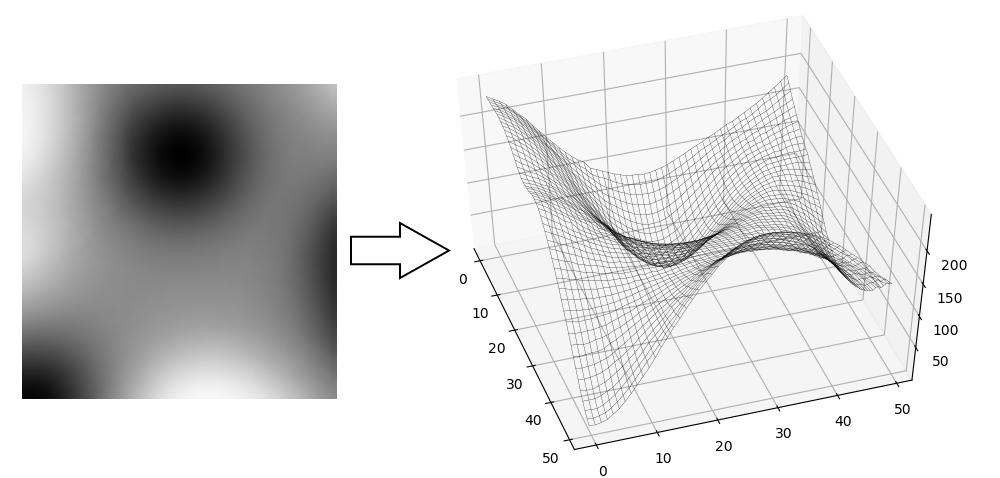
\includegraphics[width=0.58\textwidth]{img/visu1.png}
\caption{gray-scale to height-map conversion}
\label{fig:conversion}
\end{wrapfigure}

Now our aim is to partition the surface into \emph{regions} (i.e. subsets) in a particular way:
We require each region to consist only of a single slope, by which we mean that we can ascend (or descend) from any given point of the region, to any other given point of the region, along a path that runs entirely within the region.
Such a decomposition is not unique, but we can at least try to get a partition \emph{as coarse as possible}, meaning that we merge slope regions if the resulting subset is still a slope region, and we iterate this until no further change occurs.
There might be many different coarsest slope decompositions.

The criterion we used to describe slopes, any two points being connected by either an ascending or a descending path, can easily be used in higher dimensions.
Think of a computer tomography scan, which will yield gray-scale data, but not just on a 2D image, but rather on a 3D volume.
We want to partition the 3D volume, such that any two points in a region can be connected via an either ascending or descending path within the region.
Recall that \emph{ascending} and \emph{descending} refers to the brightness value of the tomography scan as we move in the volume. For piecewise linear functions on a volume, decompositions were introduced in \cite{edelsbrunner2003morse}. 

By abstracting from image and tomography to a real function $f: \Omega \rightarrow \mathbb{R}$ defined on some subset of $\mathbb{R}^n$ (think of it as the pixel intensity function), and by rigorously defining a coarsest slope decomposition, we can lift the concept to arbitrary dimensions in a mathematically concise fashion.

\section{Defining Slope Regions}
\label{sec:definitions}

%In this and the following chapters we will consider a set $\Omega \subset \mathbb{R}^n$ with $n > 1$ and a continuous function $f: \Omega \to \mathbb{R}$.

In this and the following chapters we will consider a topological space $(\Omega, \mathcal T)$ with a continuous function $f: \Omega \to \mathbb{R}$.
In practice or for ease of imagination, $(\Omega, \mathcal T)$ will typically be a rectangle or cuboid subset of $\mathbb R^2$ or $\mathbb R^3$ equipped with the euclidean topology and $f$ will describe a continuous image or 3D-scan.

\begin{defn}
A \emph{path} is a continuous function from the real interval $[a,b]$ (with $a<b$) into a topological space $\Omega$.
\end{defn}


\begin{defn}
Two points $x\neq y$ in a topological space $\Omega$ are called \emph{path-connected} if and only if there exists a path $\gamma: [a,b] \to \Omega$ with $\gamma (a)=x$ and  $\gamma (b)=y$.
\end{defn}

\begin{defn}
The set of all points which are path-connected to a point $x\in\Omega$ is the \emph{connected component of $x$}:
$$[x]:=\left\{ y\in\Omega | x ~\text{is path-connected to}~ y \right\}$$
Any subset of $\Omega$ which can be written in above way (for a suitable choice of $x$) is called a \emph{connected component}.
\end{defn}

\begin{defn}
A path $\gamma: [a,b] \to \Omega$ is called \emph{monotonic} if and only if the whole path is ascending or the whole path is descending, meaning the first or second formula below has to hold, respectively:
\begin{align*}
\forall & s, t \in [a,b]: s < t \Rightarrow f(\gamma(s)) \leq f(\gamma(t))\\
\forall & s, t \in [a,b]: s < t \Rightarrow f(\gamma(s)) \geq f(\gamma(t))
\end{align*}
\end{defn}

\begin{defn}
Let $R \subset \Omega$. $R$ is called \emph{slope region} or \emph{monotonically connected} if and only if for all $x, y \in R$ there exists a monotonic path $\gamma: [a,b] \to R$ with $\gamma(a) = x$ and $\gamma(b) = y$.
\end{defn}

\begin{defn}
A family of sets $\left\{ A_i \subset \Omega \mid i \in I \right\}$ is called a \emph{slope region decomposition} if and only if:
\begin{itemize}
\item $A_i$ is a slope region for all $i \in I$
\item $\forall i,j \in I: i \neq j \Rightarrow A_i \cap A_j = \emptyset$.
\item $\bigcup_{i\in I} A_i = \Omega$
\end{itemize}
\end{defn}

%\begin{defn}
%A slope region decomposition $\left\{ R_i \subset \Omega \mid i \in I \right\}$ is called \emph{maximally coarse} or simply \emph{coarse} if and only if there is no $J \subset I$ with $|J| \geq 2$ and
%\begin{equation*}
%\left\{ R_i \subset \Omega \mid i \in I \setminus J \right\} \cup \left\{ \bigcup_{j\in J} R_j \right\}
%\end{equation*}
%\end{defn}


\begin{defn}
Consider two slope region decompositions $\mathcal{A} = \left\{ A_i \subset \Omega \mid i \in I \right\}$ and $\mathcal{B} = \left\{ B_j \subset \Omega \mid j \in J \right\}$.
We call $\mathcal{A}$ \emph{coarser than} $\mathcal{B}$, alternativly $\mathcal{B}$ \emph{finer than} $\mathcal{A}$, in Symbols $\mathcal{A} \succeq \mathcal{B}$ if and only if
\begin{equation*}
\forall j \in J ~ \exists \, i \in I: B_j \subset A_i.
\end{equation*}
\end{defn}

\begin{thm}
$\succeq$ is a partial order, i.e. fulfills reflexivity, antisymmetry and transitivity.
\end{thm}
\emph{Proof:} Straight forward. Antisymmetry follows from the decomposition property. \hfill $\Box$

\begin{defn}
A slope region decomposition $\mathcal{A}$ is called \emph{maximally coarse} or simply \emph{coarse} if and only if there is no other coarser slope region decomposition.
\end{defn}

We can apply Zorn's lemma \cite{zorn1935remark} to the partial order $\succeq$, which yields the existence of maximal elements.
Hence every set $\Omega$ has a coarse decomposition.

\begin{thm}
\label{slope_iff_conn_lvlsets}
Let $A \subset \Omega$ be a path-connected set.
$A$ is a slope region if and only if all levelsets of $f$ in $A$ are path-connected, i.e.
\begin{equation*}
\forall c \in \mathbb{R}: f^{-1}(c) \cap A ~ \text{is path-connected}.
\end{equation*}
\end{thm}

\emph{Proof:} "$\Rightarrow$" via contraposition:

Suppose there exists a $c \in \mathbb{R}$ with $L := f^{-1}(c) \cap A$ not path-connected.
We decompose $L$ in its components and pick $x$ and $y$ from different components.
Since $f(x) = f(y) = c$ a monotonic path between $x$ and $y$ would have to lie completely in L.
However, since $x$ and $y$ are from different components, they cannot be connected by a path in $L$ and therefore cannot be connected with a monotonic path.
Therefore, A is not a slope region.

$~$

\begin{wrapfigure}{R}{0.35\textwidth}
\centering
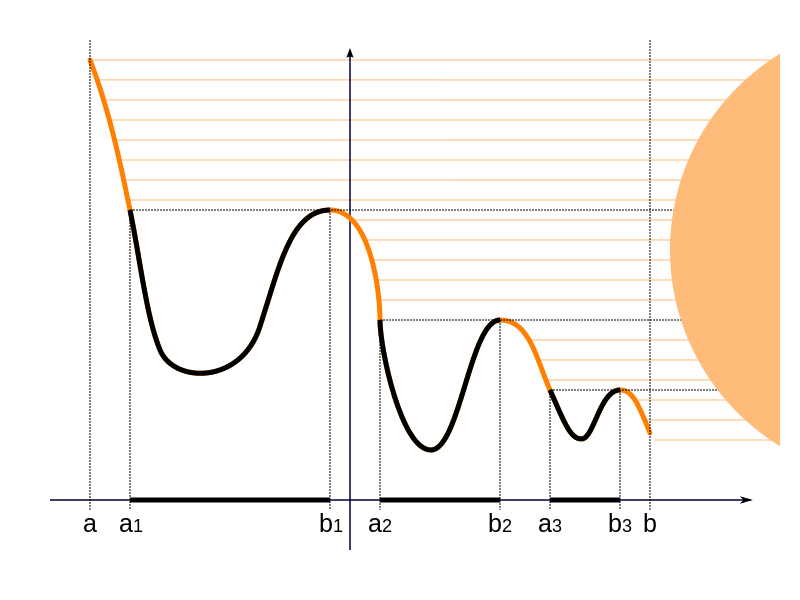
\includegraphics[width=0.35\textwidth]{img/Rising_sun_lemma.png}
\caption{Rising Sun lemma}
\label{fig:lemma_1}
\end{wrapfigure}

"$\Leftarrow$" via \emph{ironing out} an arbitrary path:

Given $x, y \in A$ we have to find a monotonic path $\gamma$.
Without loss of generality suppose $f(x) \geq f(y)$.
Since $A$ is path-connected, there exists an (not necessarily monotonic) path $\gamma_0: [a,b] \to A$ from $x$ to $y$.
Using the Rising Sun lemma \cite{riesz1932theoreme} on the continuous function $f \circ \gamma_0$ we get the \emph{shadow} $S = \bigcup_{i \in I} (a_n, b_n)$ consisting of at most countably many intervals.

$S$ consists of the points which contradict the monotony of $f \circ \gamma_0$, thus we want to \emph{iron out} these points.

Let $c_n := f(a_n) = f(b_n)$. Since the levelset of $c_n$ is path-connected, we can connect $\gamma_0(a_n)$ and $\gamma_0(b_n)$ with a level path $\gamma_n^* : [a_n, b_n] \to A.$

Finally, we define:
\begin{equation*}
\gamma(\sigma) :=
\begin{cases}
\gamma_n^*(\sigma) & \sigma \in [a_n, b_n] \\
\gamma_0(\sigma) & \text{elsewhere}
\end{cases}
\end{equation*}

$\gamma$ is a monotonic path from $x$ to $y$, thus $A$ is a slope region.
\hfill $\Box$



\section{Results In The Plane And Counterexamples In Higher Dimensions}

There are two theorems (\!\!\cite{kropatsch2019computing} Lemma 1 and \cite{kropatsch2019computing} Lemma 2) that are useful, but only hold if $\Omega \subset \mathbb R^2$, not in general if $\Omega \subset \mathbb R^d$ for $d > 2$.
But first, a lemma.

\begin{thm}
Let $A$ be a slope region.
Then the closure $\bar A$ is also a slope region.
\end{thm}

\emph{Proof:} Follows from continuity of $f$.
\hfill $\Box$

The following theorem is only formulated for closed slope regions, but because of the above theorem this is not a big restriction.

\begin{thm}
Let $d = 2$ and $A \subset \mathbb R^d$ be a closed and bounded slope region.
Let $(\partial A_i)_{i\in I}$ be an enumeration of the connected components of the boundary $\partial A$.
Then $\forall i \in I : f|_{\partial A_i}$ has at most one local minimum and one local maximum.
\end{thm}

\begin{wrapfigure}{R}{0.25\textwidth}
\centering
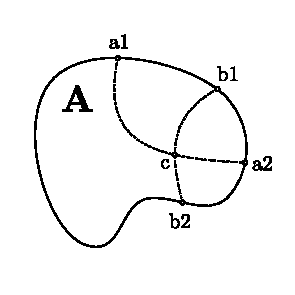
\includegraphics[width=0.25\textwidth]{img/sketch_border_thm.pdf}
%\caption{Sketch of Proof.}
\label{fig:sketch_1}
\end{wrapfigure}

\emph{Proof:} Assume there are two local minima $a_1, a_2 \in \partial A_i$ with $f(a_1) \leq f(a_2)$.
Since $\partial A_i$ is connected, there has to be a point $b_1 \in \partial A_i$ between them with $f(a_2) < f(b_1)$.
On the 'other side' of $a_2$ there has to be a point $b_2 \in \partial A_i$, also with $f(a_2) < f(b_2)$.
Note that the 'other side' exists only because $\Omega = \mathbb R^2$ and thus $\partial A_i$ is a line.

Since $A$ is a slope region, $a_1$ and $a_2$, as well as $b_1$ and $b_2$ have to be connected by a monotonic path.
Because of the Jordan Curve Theorem \cite{jordan1887cours}, these paths have to cross in a point $c \in A$.
But this yields a contradiction: $f(c) \leq f(a_2) < min(f(b_1), f(b_2)) \leq f(c)$.
Thus the assumption of the existence of two local minima has to be false.

\hfill $\Box$

\begin{exmp}
Let $\Omega = \mathbb R^3$ and $A = B_1(0,0,0)$ be the closed unit ball.
Let $f$ be the distance to the $x$-Axis. 

\begin{equation*}
f: \mathbb R^3 \to \mathbb R: (x,y,z) \mapsto \sqrt{y^2 + z^2}
\end{equation*}

The levelsets of $f$ in $A$ are either the $x$-Axis for $f \equiv 0$ or the sides of cylinders for $f > 0$.
In any case, they are connected.
Thus, by theorem \ref{slope_iff_conn_lvlsets}, $A$ is a slope region.
$\partial A$ has one connected component, which is the unit sphere.
$f|_{\partial A}$ has two local minima, which are the intersections with the $x$-Axis, $(1,0,0)$ and $(-1,0,0)$.
\end{exmp}

Thus, the previous theorem does not hold in $\mathbb R^3$.
In fact, it does not hold in any $\mathbb R^d$ for $d > 2$.
There is also no limit on the number of local minima on the surface of a slope region.

\begin{thm}
\label{thm:saddle_on_border}
Let $d = 2$ and $A \subset \mathbb R^d$ be a slope region.
Let $s \in A$ be a saddle point.
Then, $s \in \partial A$.
\end{thm}

\emph{Proof:} Assume $s$ is an interior point of $A$, which means there is a open set $U$ with $s \in U \subset A$.
$s$ being a saddle point means there is a neighborhood $V \subset U$ so that $V_- := V \cap [f < f(s)]$ as well as $V_+ := V \cap [f > f(s)]$ decompose into two or more connected components.

Pick $a_1, a_2$ from different components of $V_-$ as well as $b_1, b_2$ from different components of $V_+$.
$a_1$ and $a_2$ have to be connected by a monotonic path, but this path has to move outside of $V$ since the points are from different components of $V_-$ and by virtue of being monotonic, the path can not go through $V_+$.
Analogue for $b_1$ and $b_2$.

Again by the Jordan Curve Theorem, these to paths have to cross in some point $c$, which again yields a contradiction.

\begin{equation*}
f(c) \leq max(f(a_1), f(a_2)) < f(s) < min(f(b_1), f(b_2)) \leq f(c)
\end{equation*}

Thus the assumption that $s$ is a interior point has to be false.
\hfill $\Box$

\begin{exmp}
Let $\Omega = A = \mathbb R^3$.
Let f be the distance from the unit circle laying in the $x$-$y$-plane. 

\begin{equation*}
f: \mathbb R^3 \to \mathbb R: (x,y,z) \mapsto 
\begin{cases}
\sqrt{\left(x - \frac{x}{||\left(x,y\right)||_2}\right)^2 + \left(y - \frac{y}{||\left(x,y\right)||_2}\right)^2 + z^2} & ||(x,y)||_2 \neq 0 \\
\sqrt{1+z^2} & ||(x,y)||_2 = 0
\end{cases}
\end{equation*}

Again, let us look at the levelsets to show $A$ is a slope region.
The levelset of $f \equiv 0$ is the unit circle. For $0 < f < 1$ the levelsets are tori.
$f \equiv 1$ marks a transition and the levelset is a torus with its hole closed.
Then, for $f > 1$ the levelsets look like the exterior surface of a self intersecting torus, topologically equivalent to a sphere.
All these levelsets are connected.
Thus, $A$ is indeed a slope region.

Now consider the point $(0,0,0)$.
Along the $x$ and $y$-direction it is a local maximum, however along the $z$-direction it is a local minimum.
Thus, it is a saddle point.
Therefore, theorem \ref{thm:saddle_on_border} does not hold in higher dimensions.
\end{exmp}


\section{Motivating The Border Propagation (BP) Algorithm}
\label{sec:motivating_BP}

Now we will work our way to the central insights on which the border propagation algorithm (\emph{BP}) hinges.
Let us develop ideas for smooth (hyper-)surfaces first, and deal with discrete variants in the next section.

Slope regions can be constructed and grown in a straight-forward iterative manner by sweeping through the function values from lowest to highest. 
This is similar to the intuition employed in Morse theory\cite{MatsumotoYukio2002AitM}.
Visualize a smooth, compact 2D surface in 3D space.
We want to decompose this surface into slope regions.
Initially, our decomposition is empty, i.e. there are no slope regions (thus we don't have an actual \emph{decomposition} yet).
This is shown in Figure \ref{fig:evolution}, Image 1.

\begin{wrapfigure}{R}{0.3\textwidth}
\centering
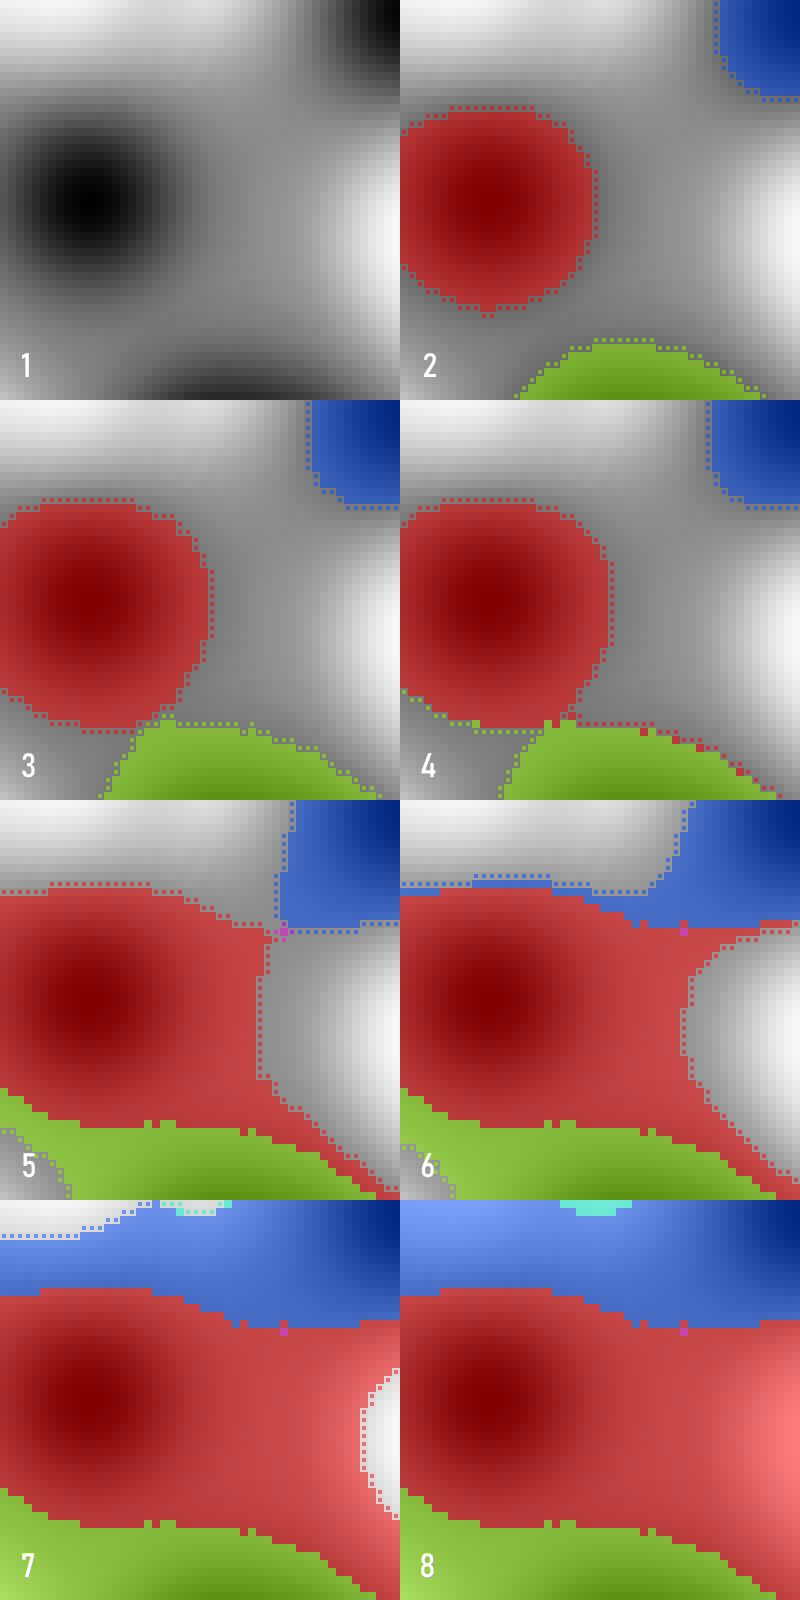
\includegraphics[width=0.3\textwidth]{img/slope_evolution.png}
\caption{evolution of discretized regions during the algorithm}
\label{fig:evolution}
\end{wrapfigure}

Imagine a water level rising from below the surface, up to the point of first contact.
Starting at this global minimum, we add a new region, containing only the argmin (i.e. a single point on the 2D image where the minimal value is taken).

Now, there might be many points where the global minimum is taken.
This will either be due to a flat region (\emph{plateau}) on the surface, which we want to include into the single existing region, or it will be due to individual dales, which all have their lowest point at the same height.
In this case, we can't put the points into the existing region, because we would not be able to get from one argmin to another via a monotonic path.
Instead, we need to add a new region for each individual dale.

Both cases can be dealt with by contracting connected points into their connected component, and creating a new region for each resulting component. This will ensure that plateaus are assigned to a single region.

As the water rises, we can add points to an existing region growing it upwards if they are just outside the region\footnote{Why can we do that?
By adding only points which are connected to the region we ensure path-connectedness, and by growing the region upwards, we can construct ascending paths from old points to new ones.
The smoothness of the surface guarantees that while moving at a fixed height, we can reach all points of the region with that height.}.
Otherwise they correspond to a distant local minimum and have to be dealt with as before, by opening a new region for each point (or rather, each connected component).
This is shown in Figure \ref{fig:evolution}, Image 2.

With the water rising further still, the regions will grow upwards to a point where they meet (Figure \ref{fig:evolution}, Image 3).
Any such point is a saddle point, and we have to account for it the next time we want to grow any one of the touching regions.
The saddle point connects the edges of the regions which meet in it, at the current height of the water level.
It might be the case that the not-yet-assigned points (the ones above the water) get separated into multiple connected components, or they might remain connected.

If the points remain connected, then we have to decide for a single one of the involved regions to be allowed to grow upwards from the component.
This means that one region effectively inherits the growth directions from the other region(s).
The other region(s) lose their potential for expansion and remain frozen in their current state.

If the unassigned points have multiple components (as in Figure \ref{fig:evolution}, Image 3: the unassigned grey points are separated into the lower left and upper right areas), then we may assign one component to each involved region.
The regions will then grow only in the directions determined by the assigned components as the water rises.
This can be observed in Figure \ref{fig:evolution}, Image 4: The green region is allowed to grow to the lower left, while the red region floods the upper right.
The same procedure of swapping areas of expansion also happens as we move from Image 5 to 6.
Any region without an assigned component remains frozen.
Should there be more components than regions, then we open up a new region for each surplus component, as in the top of Image 7.

An oddity which can occur are self-loops: A region might grow into a "C"-shape, and then proceed to close up into an "O"-shape.
This case can be treated similarly as above, the only difference is that the saddle is found by recognizing that the region collides with itself, not with another region.

Eventually this procedure will arrive at the global maximum, and the entire surface will be divided into regions.
Since we proceeded with the necessary care and attention along the way, we ensured that the regions remained slope regions, and we also only created additional regions when we absolutely had to, showing that the resulting composition is maximally coarse.

The same algorithm can be applied in higher dimensions.
We deal with iso-hyper-surfaces as level sets, but the topological considerations about connectedness remain the same as in the illustrative 2D case.

\section{Discrete BP}
\label{sec:details}

The somewhat vague description of BP in the previous section assumed a continuous surface.
In most applications, however, the data will be provided in a discrete raster format.
Some intricacies arise from this discretization, most notably iso-surfaces of a smooth function $f$ will not have a straight-forward representation in the discrete grid obtained from rasterizing $f$.
The data structure we use is a set of indices, representing the positions in the discrete array already assigned to a region.

Each region also has a set of (yet) unassigned points, which determine where the region might grow in the next iteration, called the \emph{border}.
This effectively models the smooth levelsets in the discrete representation.

The pseudo-code for the algorithm is printed below, the executable python code can be accessed in our github repository:
\url{https://github.com/SirFloIII/MustererkennungLVA}

\begin{algorithm}
\caption{Border Propagation}
\begin{algorithmic}
\State Enumerate all values of $f$ and collect points into levelsets.
\For{each levelset in bottom to top order}
    \State Add points to regions if they are in the border of a region
    \If{an added point is in the border of different region}
        \State Find the union of the borders of the involved regions
        \State Find the connected components thereof
        \State Assign these to the regions in an arbitrary way
	\EndIf
    \If{an added point splits the border of the region in two}
        \State Reduce the border the region to one component
        \For{each other component}
            \State Create a new region containing the component as border
		\EndFor
    \EndIf
    \For{leftover points that cannot be added to any regions}
        \State Create a new region containing only that point
	\EndFor
\EndFor
\end{algorithmic}
\end{algorithm}

%As a result, there are multiple ways to define what a \emph{discrete slope region} is supposed to be.
%Let us first explore, why the most obvious choice for a definition does not characterize the property we are interested in.
%Using the discrete notion of connectedness, allowing discrete paths to move only axially (or at best diagonally) each step, one can define a slope region:
%$R$ is a slope region iff any two points in $R$ can be connected via a monotonic discrete path contained in $R$.
%
%There is a simple example to demonstrate that this definition is a bad one: Imagine a 2D plane, which is at a slant in 3D space, such that it isn't parallel to any of the 3 axes.
%For instance the graph of the function $f: \mathbb{R}^2 \rightarrow \mathbb{R}: (x,y)\mapsto x+y$.
%Clearly a sensible slope decomposition would assign the entire plane to a single region.
%But let's look at what happens after discretization.
%Points representing a single continuous levelset will not be directly adjacent to each other on the discrete grid, but diagonally adjacent at best.
%Depending on the discretization of the function values, a single levelset might consist of points even more dispersed than that.
%Each point will be considered an individual connected component of the region border and many new regions will be generated, even though we know that on the continuous surface the points belong to a single levelset.
%
%It is precisely this realization that led us to the BP algorithm.
%Every region consists of the points already added to it, but the region also remembers its \emph{halo}, which is a set of unassigned points directly (axially, not diagonally) adjacent to the region points.
%The halo can be seen as the direction into which the region is allowed to expand.
%This data structure models the continuous level set connectedness.
%In Figure \ref{fig:evolution} the halo of a region is shown as tiny dots of the same color as the region.
%
%The search for the connected components of a level set in the continuous case corresponds to the search of connected components of the halo in the space of all unassigned points.
%This search is computationally expensive and would have to be performed whenever a point is assigned to a region, which is why a very fast test is done first:
%Only if the halo is disconnected within a small local environment, a global test is performed.
%
%Much like connected components need to be assigned to colliding regions in the continuous case, the same has to be done in the discrete world.
%BP achieves this by distributing halo components among the involved regions.
%The heuristic chosen by the authors to decide which region gets which component during a halo swap is as follows:
%The component which allows for expansion towards the biggest chunk of unassigned points gets assigned to the involved region with the lowest minimum.
%The component allowing for second largest expansion gets assigned to the involved region with the second lowest minimum, etc.
%The intent is to prefer the construction of large regions which reflect the topology well, and to freeze tiny regions, since they have a good chance of resulting from noise.


%By iterating over the levelsets and swapping entire halo components, BP effectively ensures that the borders between regions are on the discretized equivalent of a continuous levelset.
%This property allows for an interesting characterization related to Reeb Graphs, as shown in the next section.

%\section{Slope Decompositions From Reeb Graph}
%\label{sec:reeb}
%
%\begin{wrapfigure}{R}{0.25\textwidth}
%\centering
%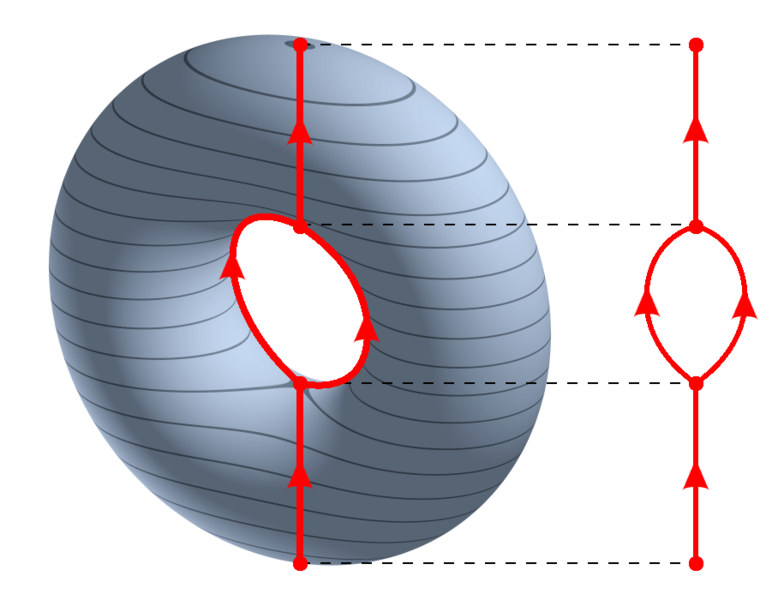
\includegraphics[width=0.25\textwidth]{img/Reebgraph.png}
%\caption{Reeb graph of the torus}
%\label{fig:reeb_torus}
%\end{wrapfigure}
%
%
%There is a significant connection between Reeb graphs and slope region decompositions.
%
%
%\begin{defn}
%Let $(\Omega, \mathcal T)$ be a topological space, and $f: \Omega \to \mathbb R$ continuous. We define an equivalence relation for $x,y \in \Omega$: 
%\begin{equation*}
%x \sim y :\Leftrightarrow f(x) = f(y) = c ~\land ~ x ~\text{and}~ y ~\text{are path-connected in}~ f^{-1}(c)
%\end{equation*}
%The \emph{Reeb graph} of $\Omega$ is $G := \Omega/_\sim$
%\end{defn}
%
%\begin{exmp}
%Let $\Omega$ be a torus on its side and $f$ be the distance from the ground.
%Its Reeb graph is depicted in Figure \ref{fig:reeb_torus}.
%\end{exmp}
%
%In general, a Reeb graph consists of vertices and lines between them.
%Vertices correspond to critical points of $f$.
%They are local extrema iff their rank is $1$ and saddle points iff their rank is bigger than $2$.
%
%\begin{thm}
%Let $S$ be a slope region.
%$S/_\sim$ may intersect no more than one point of $G$ at a given height.
%
%\emph{Proof:} Follows from Theorem \ref{slope_iff_conn_lvlsets}.\hfill $\Box$
%\end{thm}
%
%Conversely:
%
%\begin{thm}
%Let $L$ be a connected linear subset of $G$.
%$S := \bigcup_{l \in L} l$ is a slope region with the additional property that its borders are along levelsets.
%
%\emph{Proof:} Also follows from Theorem \ref{slope_iff_conn_lvlsets}.\hfill $\Box$
%\end{thm}
%
%Thus, decompositions of a Reeb graph $G$ into connected linear subsets of $G$ are isomorphic to slope region decompositions with borders along levelsets, which are exactly the kind of slope region decompositions which BP produces.



%\section{BP And Other Segmentation Methods}
%\begin{itemize}
%\item BP might be considered a \href{https://en.wikipedia.org/wiki/Level-set_method}{level set method}.
%\item Even though the algorithm was motivated using a rising water surface, it is indeed very different from the seemingly similar \href{https://en.wikipedia.org/wiki/Watershed_(image_processing)}{watershed algorithm} both in its mechanics and resulting segmentation. Watershed searches for drainage basins, and a drainage basin can contain multiple coarse slope regions. (Consider a bumpy hillside.) A slope region can also be spread over multiple drainage basins. (Consider a mountaintop which is a slope region, but whose ridge is the border between drainage basins.)
%\item Much like \href{https://en.wikipedia.org/wiki/Maximally_stable_extremal_regions}{maximally stable extremal regions method}, regions are grown around extrema in BP. But slope regions do not have to be extremal (in the sense that either all points in the region are above any point on the border, or all points are below), and neither is their border maximally stable. In fact, borders of slope regions will change quite drastically by sliding them up or down, as they will change their topology by passing a saddle point.
%\end{itemize}


\section{Further Potential Development}
The result of BP is satisfactory, but we assume that improvements can be made in running time.
The code was profiled multiple times and has been adapted to run faster with significant gains in many instances.

%Most of the CPU cycles are spent searching for connected components (as of writing this document).
%We have already put efficient preliminary tests into place in order to minimize the calls to these expensive searches.
%Yet two runtime improvements come to mind:
%\begin{itemize}
%\item Growing regions not by a random choice from their halo, but from a priority queue, with new halo points being added to the end of the queue.
%This will reduce cases where self-collisions of regions are triggered, which require a call to the expensive search in order to be handled correctly.
%\item Making the expensive search itself more efficient:
%Searching for components with the A* algortihm, and encouraging the search to move along iso-surfaces.
%This will terminate the search far earlier in cases where there is only one component to be found, potentially reducing the complexity by one order for such calls.
%This optimization is being implemented as of writing.
%\end{itemize}

Additional features we consider:
\begin{itemize}
%\item Generating the Reeb graph from the slope region decomposition.
\item Providing a \emph{tolerance} parameter, which governs how steep a continuous function might get, before an iso-surface is deemed disconnected in the discrete data.
This would allow for a trade-off between continuous connectedness and discrete connectedness.
Modeling continuous connectedness creates fewer slope regions and yields pleasing results on smooth data, but the resulting regions are not monotonically connected (in the discrete sense of \emph{connected}) in general.
Discrete connectedness guarantees monotonic connectedness, but it necessarily creates significantly more and smaller slope regions.
On smooth data the latter tends to produce too fine of a decomposition.
\item Using established data structures that model smooth level sets from discrete data. There might be performance gains in employing such a data structure.
\end{itemize}

%Another interesting experiment would involve generating the Reeb Graph via an external library, dissecting it to generate a slope region decomposition, and then pitting the resulting algorithm against BP.
%Let the games begin!

%\section{Authors' Individual Contributions}
%The BP algorithm as well as this paper are the result of a pattern recognition course held at the \href{https://www.tuwien.at/en/}{Vienna University Of Technology} from Oct 2019 till Jan 2020. Professor \textsc{Kropatsch} introduced us to the concept of slope regions and posed the challenge to compute them in high dimensions ($>2$). Initially both authors were tasked with small building blocks for this endeavor:
%
%\textsc{Alex Palmrich} was to develop and implement a recognizer for saddle points, for which he coded a framework to perform efficient local regression of arbitrary degree on grid-sampled functions in arbitrary dimension. The gradient of the regression function was used to determine singular points, while the eigenvalues $\lambda_i$ of the hessian matrix provided a classification of singular points into minima (all $\lambda_i>0$), valleys (some $\lambda_i=0$, the rest positive), degenerate points (all $\lambda_i=0$), saddles (some $\lambda_i$ positive, some negative), ridges (some $\lambda_i=0$, the rest negative) and maxima (all $\lambda_i<0$). This approach turned out to be difficult to use in practice, as there were many parameters to choose, and the recognizer proved very sensitive to noise despite the smoothing resulting from regression over a big local environment. As such this fairly finished project was dropped in favor of developing BP.
%
%\textsc{Florian Bogner} was designing an algorithm similar to BP that assumed information about critical points as a given. It was supposed to use \textsc{Palmrich}'s recognizer in practice. However, as the recognizer wasn't perfect, it never reached satisfactory results and was also shelved, and energy was directed to the joint development of BP.
%
%Most of the theory behind BP as well as the actual code was conceived in direct interaction between both authors. Only some tidbits might be attributed to a single one of them, such as \textsc{Bogner}'s idea to swap halo components between regions, his proof of theorem \ref{slope_iff_conn_lvlsets}, or his code to generate an interactive display of the algorithm at work using pygame as well as chapters \ref{sec:definitions} and \ref{sec:reeb}. \textsc{Palmrich} can be credited with the use of the halo data structure, the idea of moving along iso-surfaces for a speedup during the search of connected components, and chapters \ref{sec:motivating_slope_regions}, \ref{sec:motivating_BP} and \ref{sec:details} in this paper.

\section{Conclusion}
In this paper we have shown that slope regions of continuous functions in high dimensions ($n\geq 3$) do not have the same critical point properties well-established in 2D.
Hence previous graph-based methods of building slope region decompositions by merging regions according to their border extrema will fail in high dimensions.
Instead we developed a new, levelset-based method of growing regions, which yields slope region decompositions on discrete data of arbitrary dimension.
%We assume the data to be discretized from a continuous function.

\bibliography{lit}
\bibliographystyle{plain}
\end{document}
































